\documentclass[a4paper,12pt]{article}
\usepackage[utf8]{inputenc}
\usepackage[T1]{fontenc}
\usepackage[brazil]{babel}
\usepackage{graphicx}
\usepackage{geometry}
\usepackage{amsmath}
\usepackage{float}
\usepackage{booktabs}
\usepackage{caption}
\usepackage{subcaption}

\geometry{left=3cm, right=2cm, top=3cm, bottom=2cm}

\title{Seleção de Estrutura e Validação de Modelos}
\author{Eduardo Carvalho}
\date{\today}

\begin{document}

\maketitle

\section{Análise de Amostragem e Seleção de Entradas}

\subsection{Determinação do Tempo de Amostragem}
Para a identificação dinâmica da temperatura $T_4$ (centro da câmara), analisou-se inicialmente a constante de tempo do sistema. Através da análise de autocorrelação, determinou-se o ponto onde a correlação decai para $1/e$.

\begin{itemize}
    \item \textbf{Constante de Tempo Estimada ($\tau$):} $1089.60$ s
    \item \textbf{Tempo de Amostragem Original ($T_s$):} $0.8$ s
\end{itemize}

Seguindo o critério de ter aproximadamente 4 amostras dentro de uma constante de tempo para evitar superamostragem excessiva na identificação, o tempo de amostragem alvo foi calculado em aproximadamente $272.40$ s.

Consequentemente, aplicou-se um fator de decimação de \textbf{340}, resultando em um novo tempo de amostragem de:
\[ T_{s,novo} = 272.00 \text{ s} \]

A Figura \ref{fig:decimacao} apresenta a autocorrelação utilizada para a estimativa e a comparação entre os dados originais e os dados decimados.

\begin{figure}[H]
    \centering
    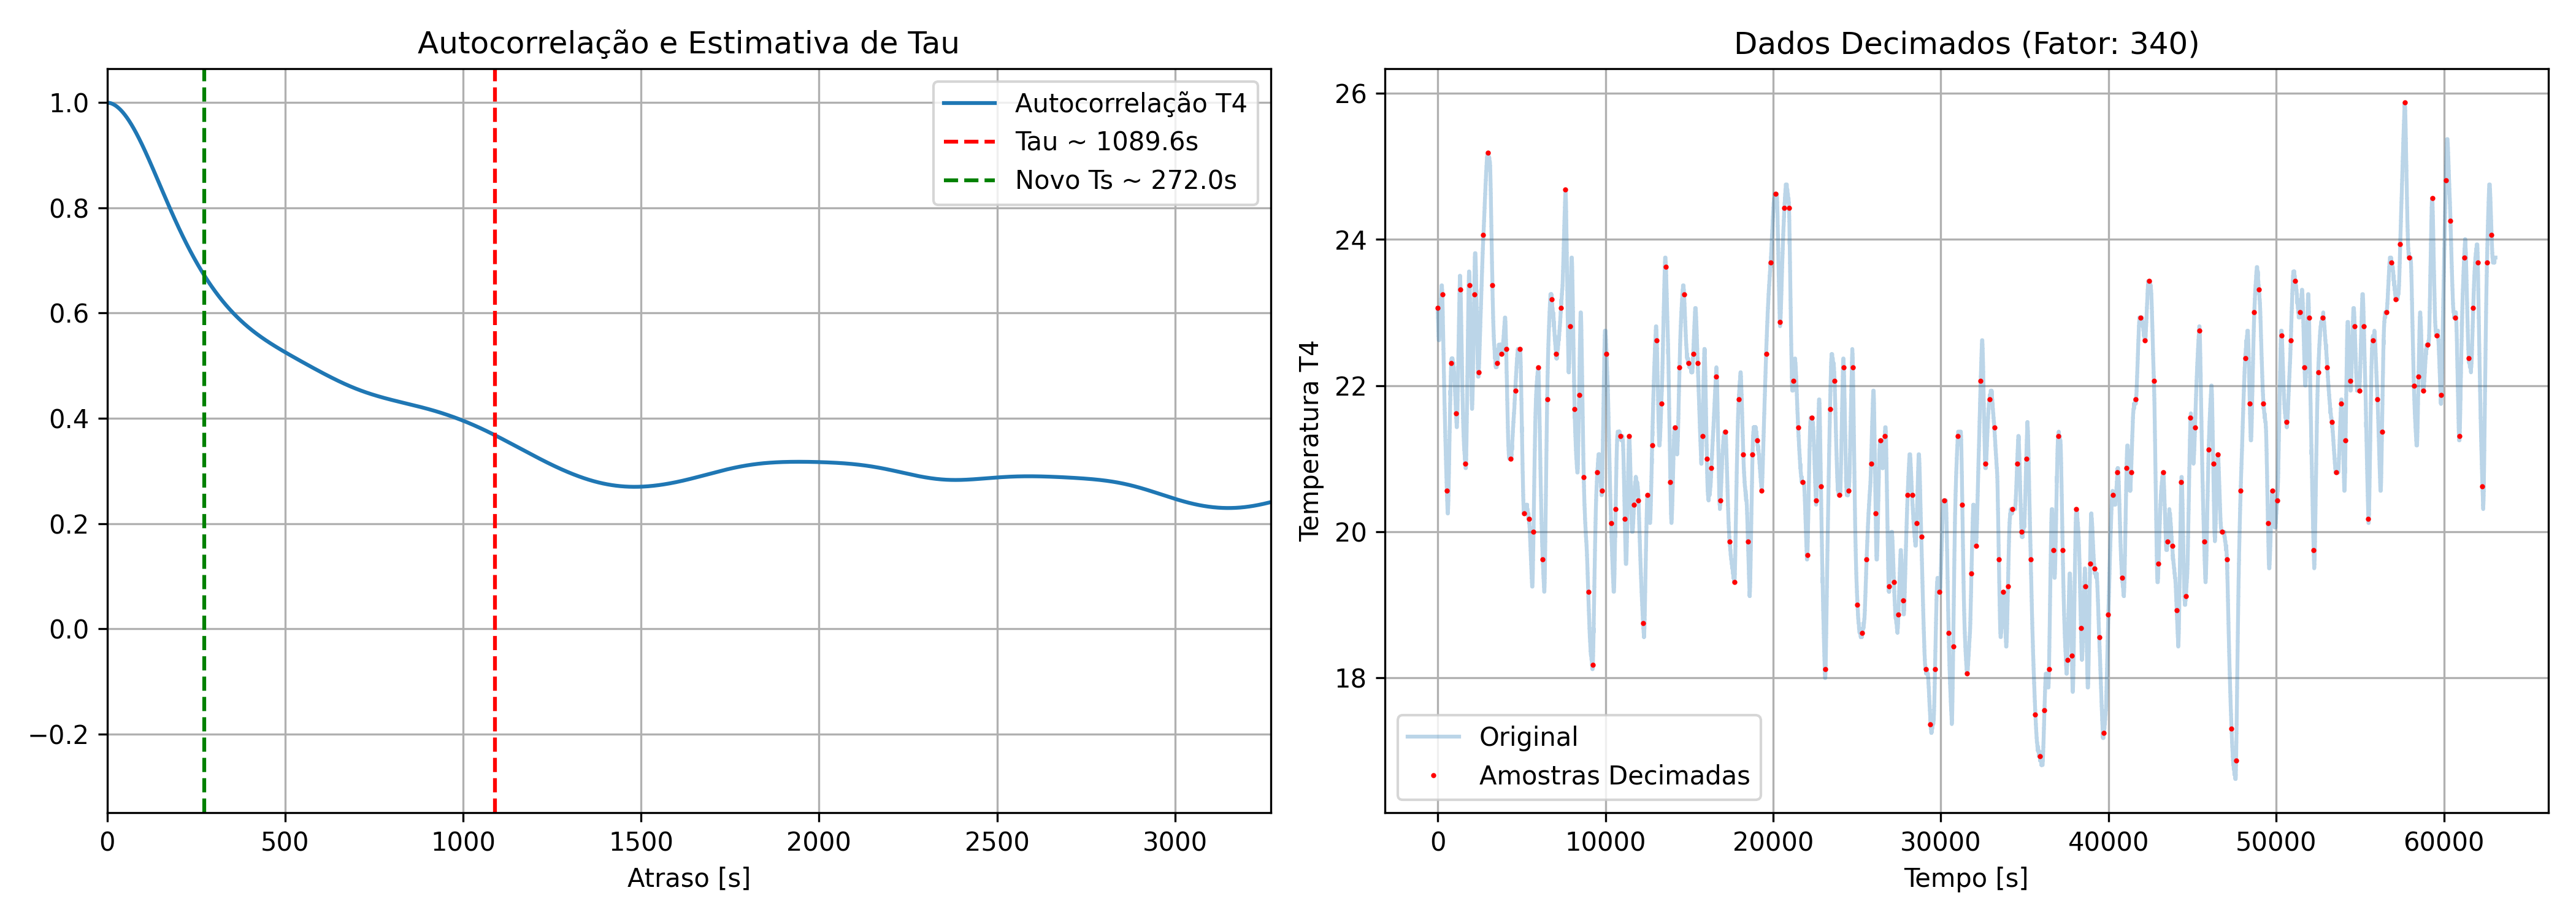
\includegraphics[width=\textwidth]{../decimacao.png}
    \caption{Autocorrelação para estimativa de $\tau$ e visualização dos dados decimados.}
    \label{fig:decimacao}
\end{figure}

\subsection{Seleção de Variáveis de Entrada}
Para definir as entradas do modelo dinâmico de $T_4$, avaliou-se a correlação entre as variáveis disponíveis. A matriz de correlação (Figura \ref{fig:correlacao}) revelou que as temperaturas $T_1$ e $T_2$ possuem altíssima correlação com a saída desejada $T_4$ (acima de 0.94).

No entanto, $T_1$ e $T_2$ apresentaram uma correlação mútua de $0.9981$. Para evitar problemas de multicolinearidade e redundância no modelo, optou-se por manter apenas a variável com a maior correlação direta com o alvo.

\textbf{Entradas Selecionadas:}
\begin{itemize}
    \item Temperatura $T_2$ - Selecionada por apresentar a maior correlação com $T_4$ e eliminar a redundância de $T_1$.
\end{itemize}

\begin{figure}[H]
    \centering
    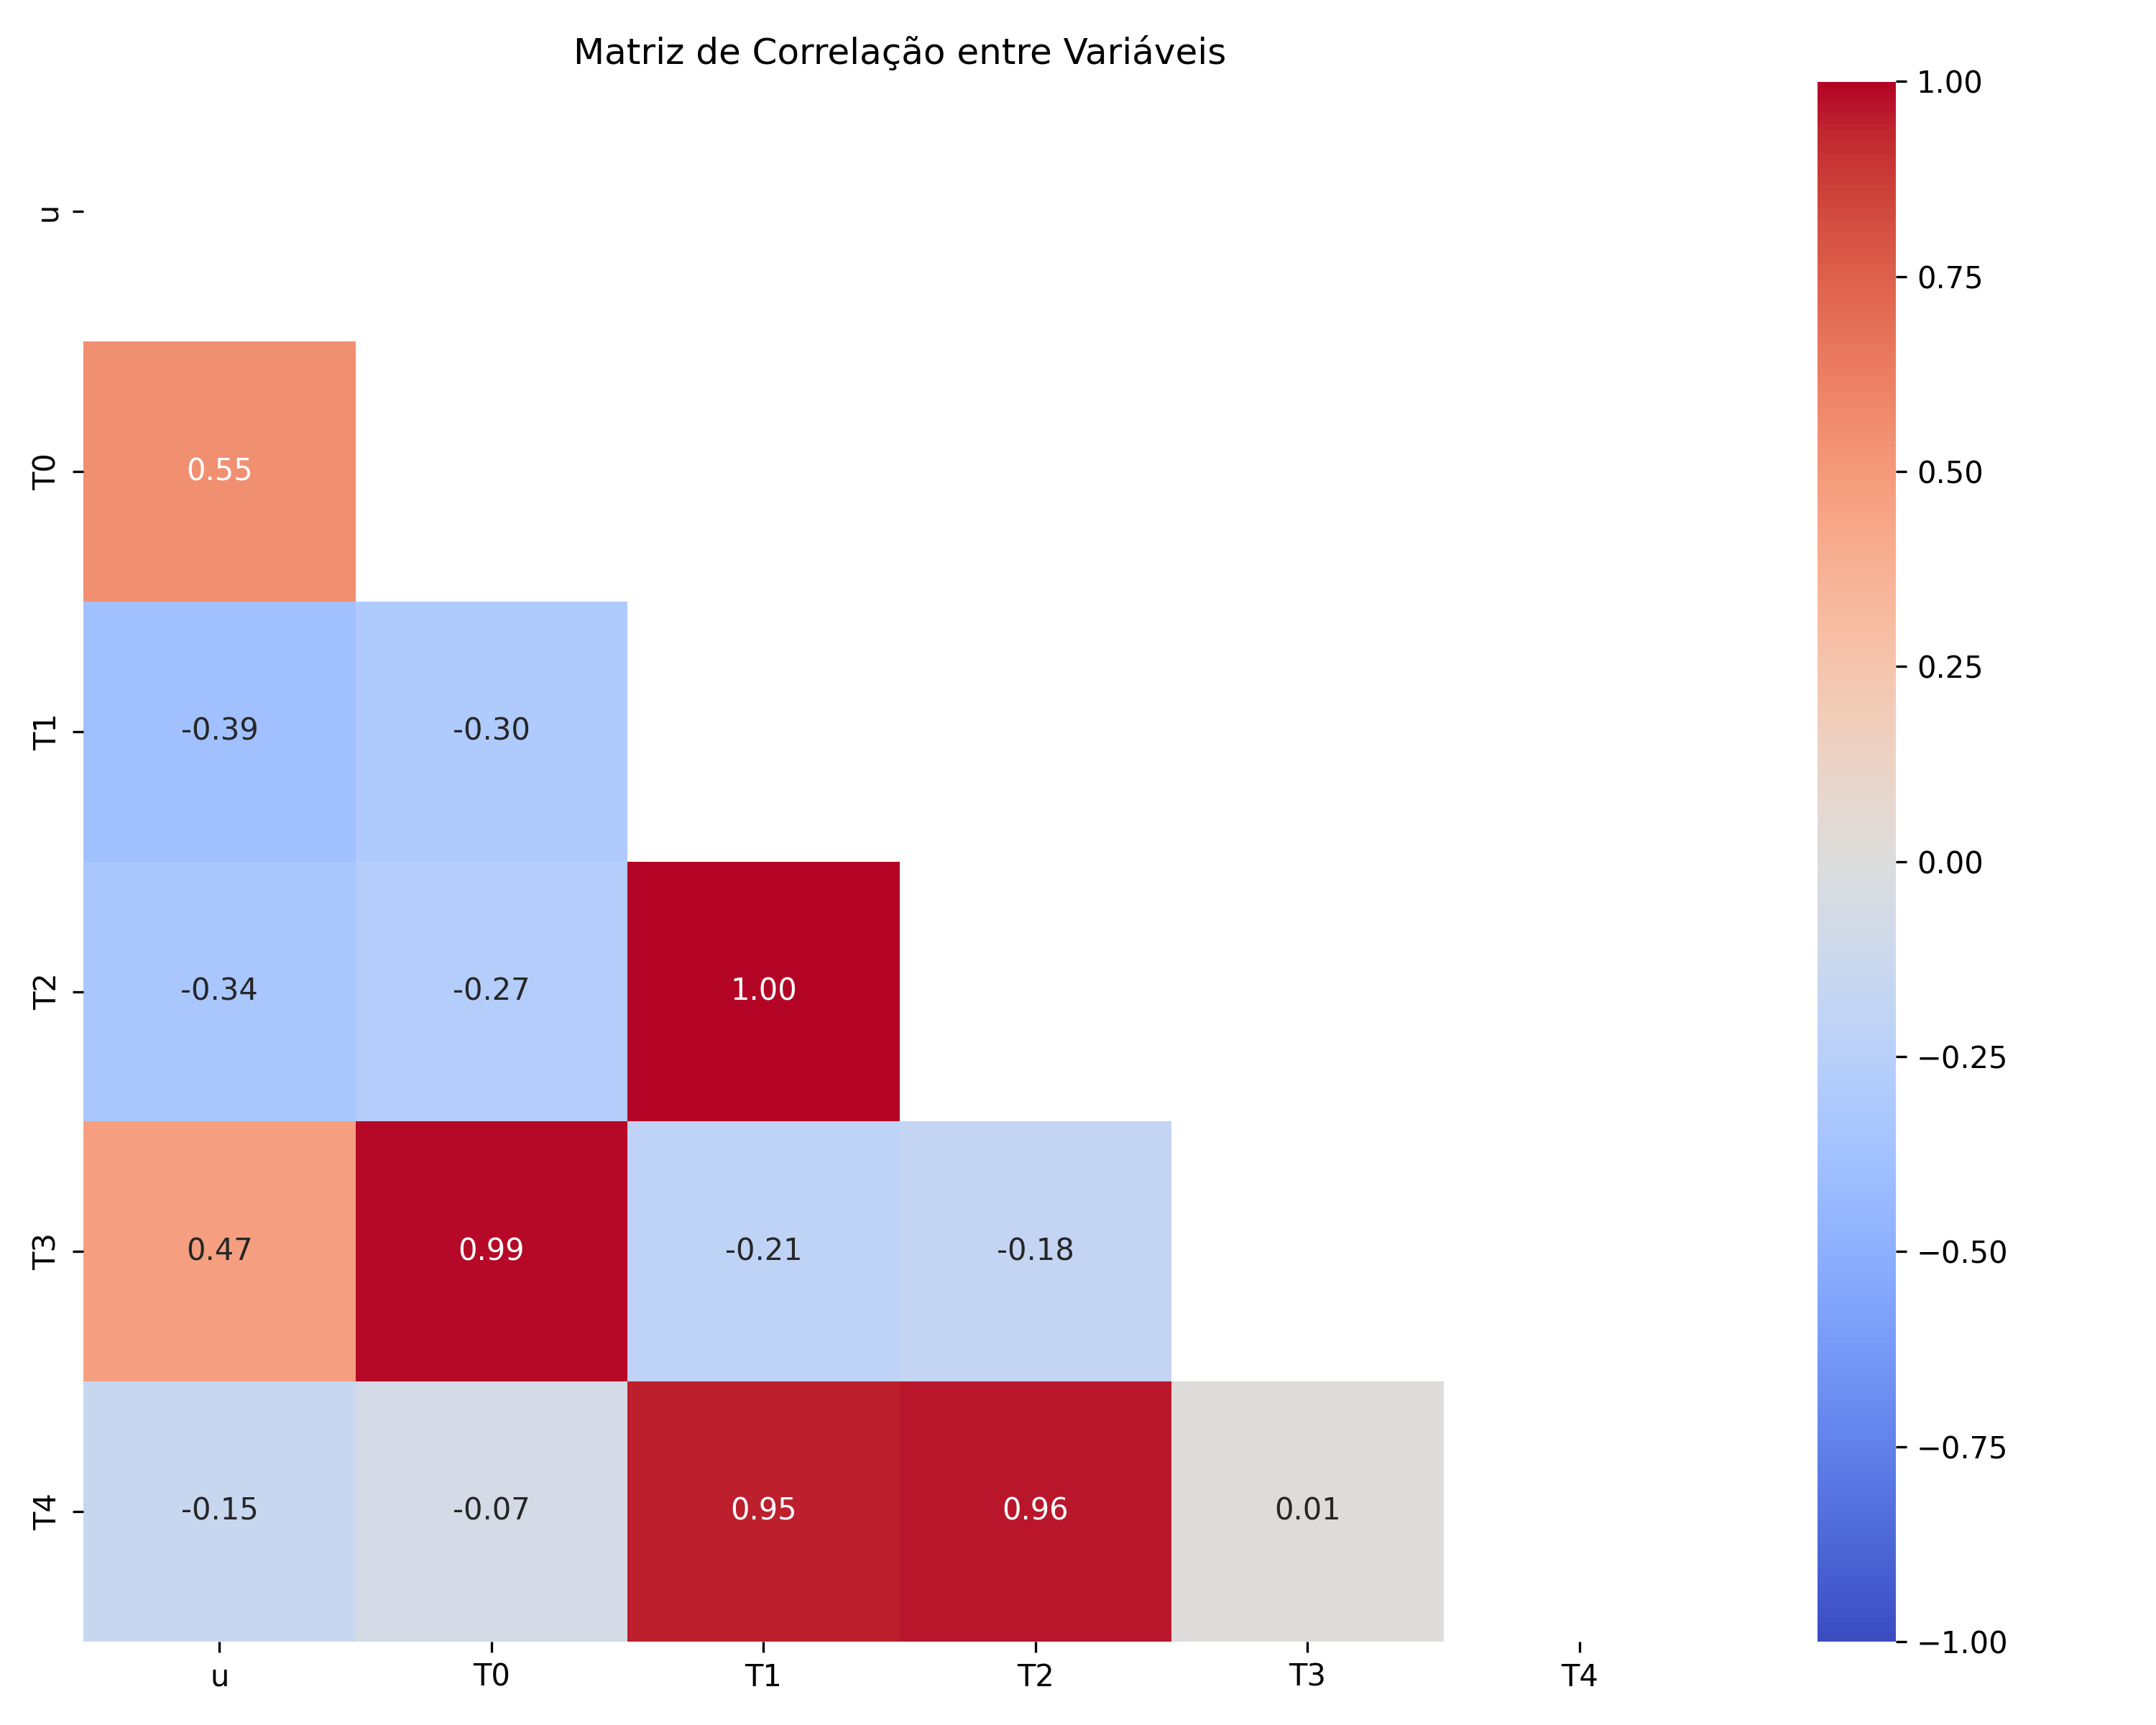
\includegraphics[width=0.8\textwidth]{../matriz_correlacao.png}
    \caption{Matriz de correlação utilizada para análise de relevância e redundância.}
    \label{fig:correlacao}
\end{figure}

\section{Identificação e Validação de Modelos}

\subsection{Divisão dos Dados}
O conjunto de dados decimado foi dividido temporalmente em três partes para garantir uma avaliação justa dos modelos: Teste (para seleção de estrutura), Treinamento (para estimação de parâmetros) e Validação (para comparação final).

\begin{itemize}
    \item \textbf{Teste:} 15\% das amostras.
    \item \textbf{Treinamento:} 60\% das amostras.
    \item \textbf{Validação:} 25\% das amostras.
\end{itemize}

\begin{figure}[H]
    \centering
    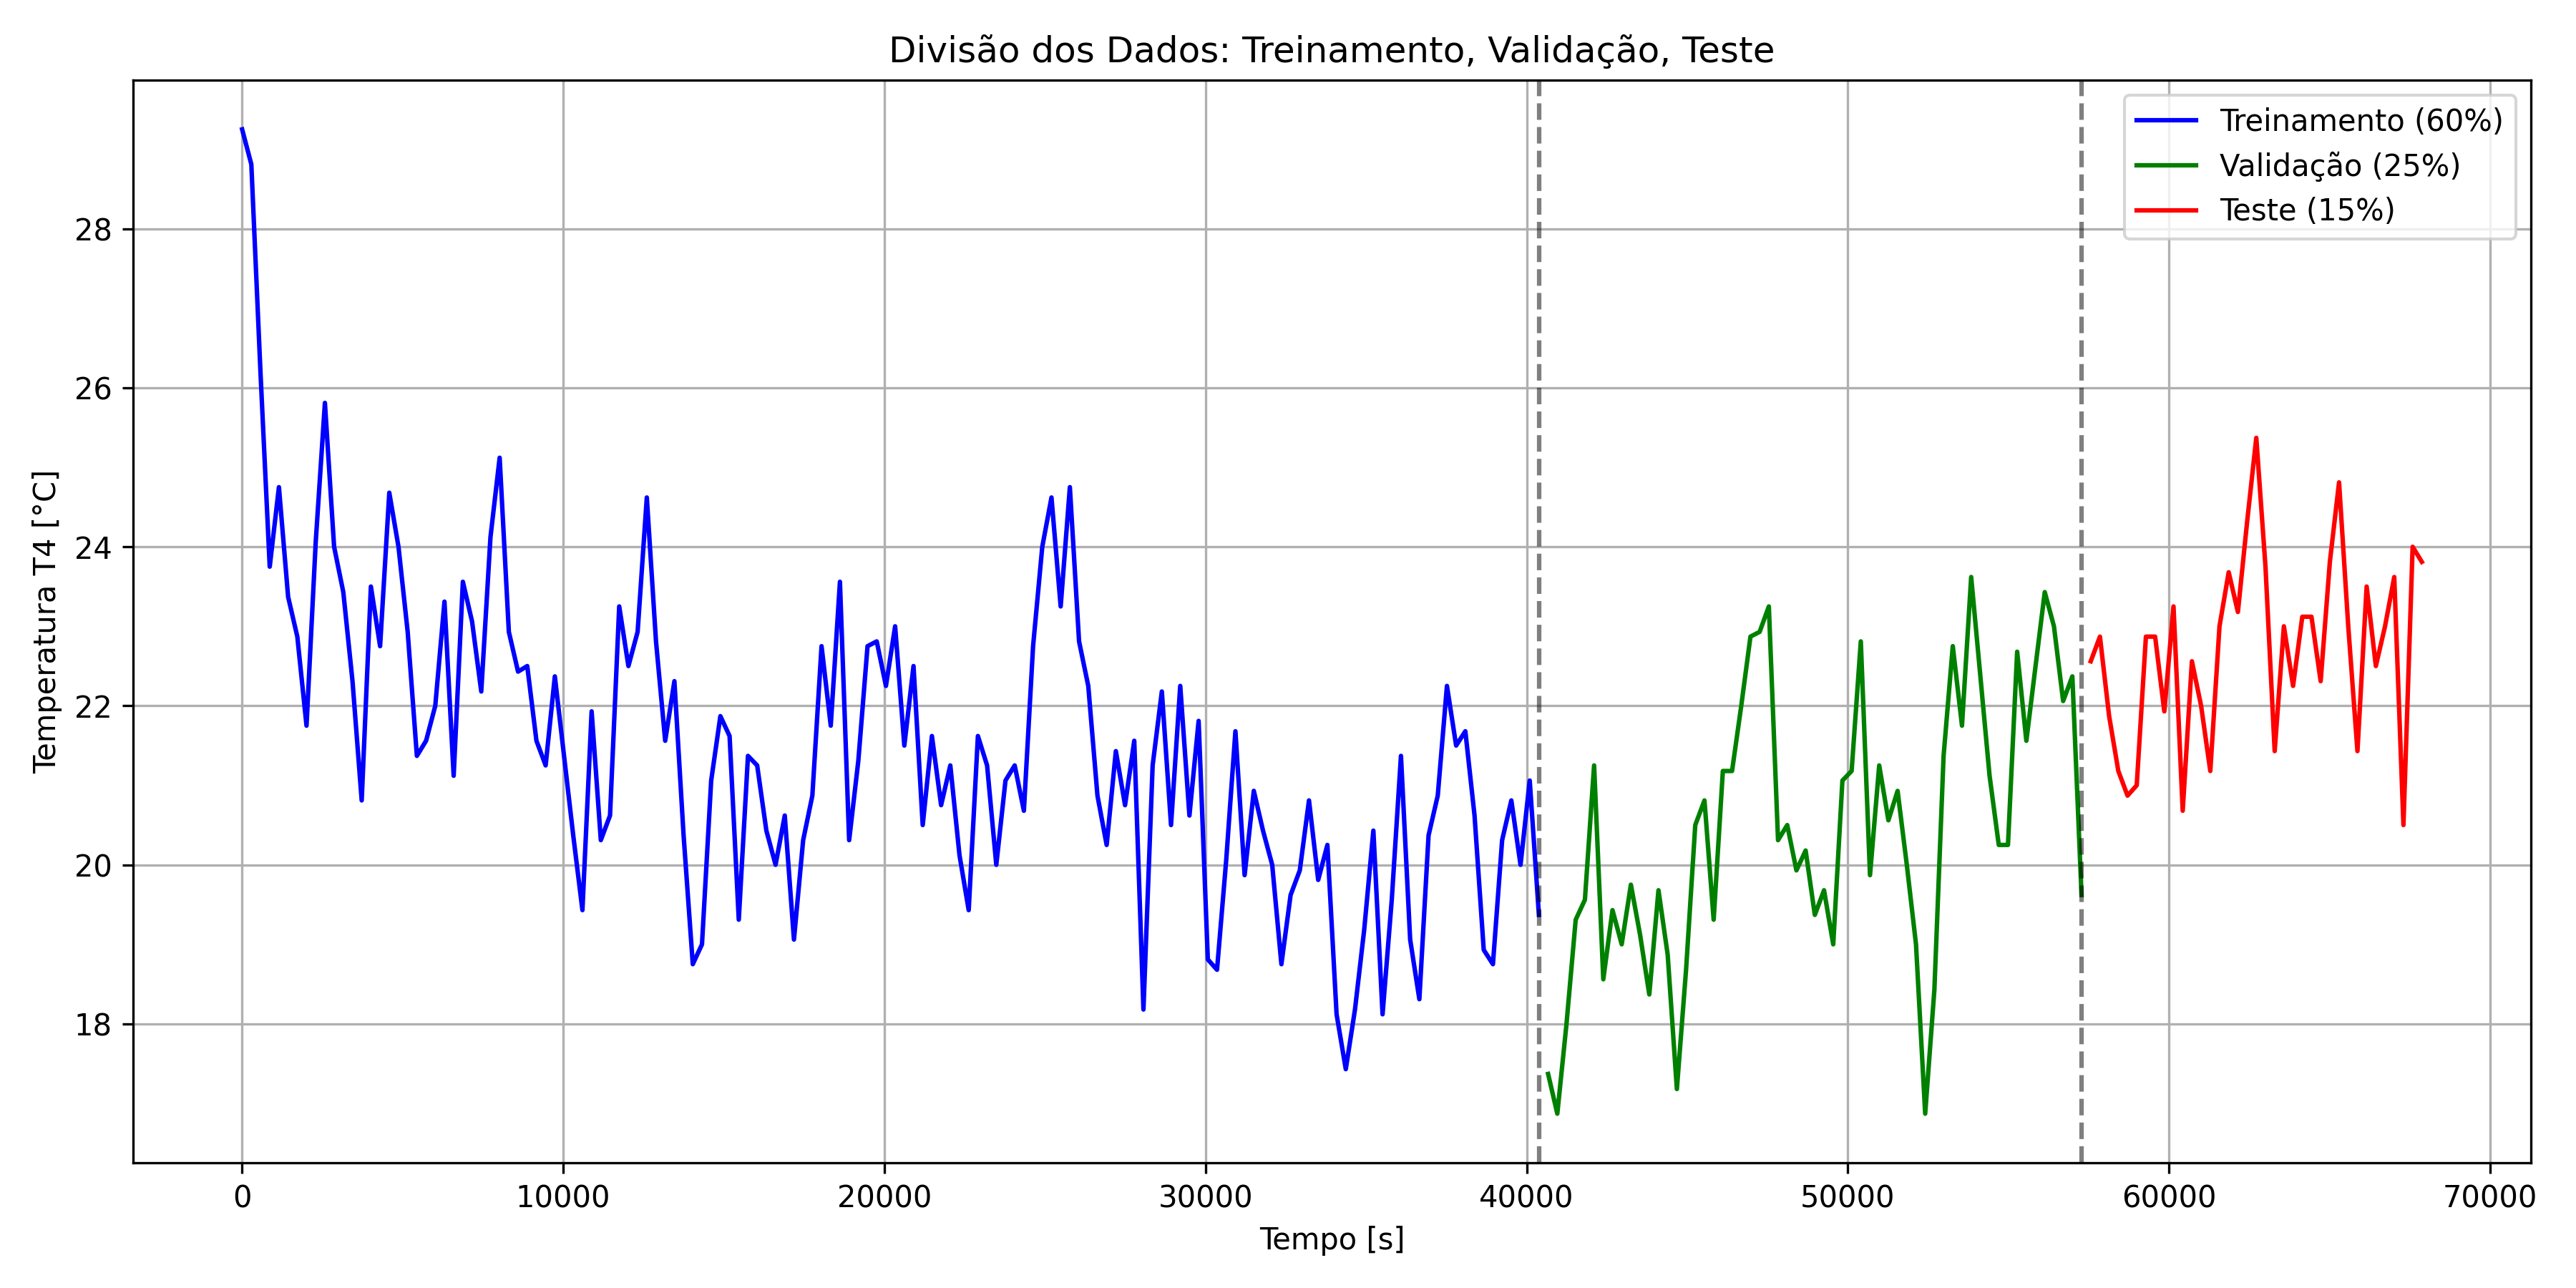
\includegraphics[width=\textwidth]{../divisao_dos_dados.png}
    \caption{Divisão temporal dos dados para as etapas de identificação.}
    \label{fig:divisao}
\end{figure}

\subsection{Determinação de Estrutura e Estimação}
Utilizando o conjunto de Teste, determinou-se a estrutura para três classes de modelos. Posteriormente, os parâmetros foram estimados usando o conjunto de Treinamento via Mínimos Quadrados.

\begin{enumerate}
    \item \textbf{Modelo Linear (ARX vs ARMAX):}
    Através do Critério de Informação de Akaike (AIC), comparou-se estruturas ARX e ARMAX.
    \begin{itemize}
        \item O modelo \textbf{ARMAX} obteve o melhor desempenho relativo, com ordem $(p=1, q=1)$ e AIC de 57.23, superando a estabilidade da predição livre do modelo ARX de ordem (1, 6).
    \end{itemize}

    \item \textbf{Modelo Não-Linear Polinomial:}
    A estrutura foi selecionada via algoritmo de Taxa de Redução de Erro (ERR). Os termos mais significativos selecionados foram:
    \begin{itemize}
        \item $y(k-1)$
        \item $u(k-1)^2$ (Termo quadrático da entrada)
        \item $y(k-2)$
    \end{itemize}

    \item \textbf{Modelo Fuzzy Takagi-Sugeno:}
    Utilizou-se o algoritmo Fuzzy C-Means para determinar os antecedentes. A análise do coeficiente de partição (FPC) indicou que \textbf{2 clusters} (regras) proporcionam a melhor separação para este conjunto de dados.
\end{enumerate}

\subsection{Análise de Resíduos}
A análise dos resíduos (Figura \ref{fig:residuos}) mostra que os modelos ARMAX e Fuzzy apresentaram distribuições de erro mais próximas de uma normal e com menor variância. O modelo ARX apresentou desvios mais significativos.

\begin{figure}[H]
    \centering
    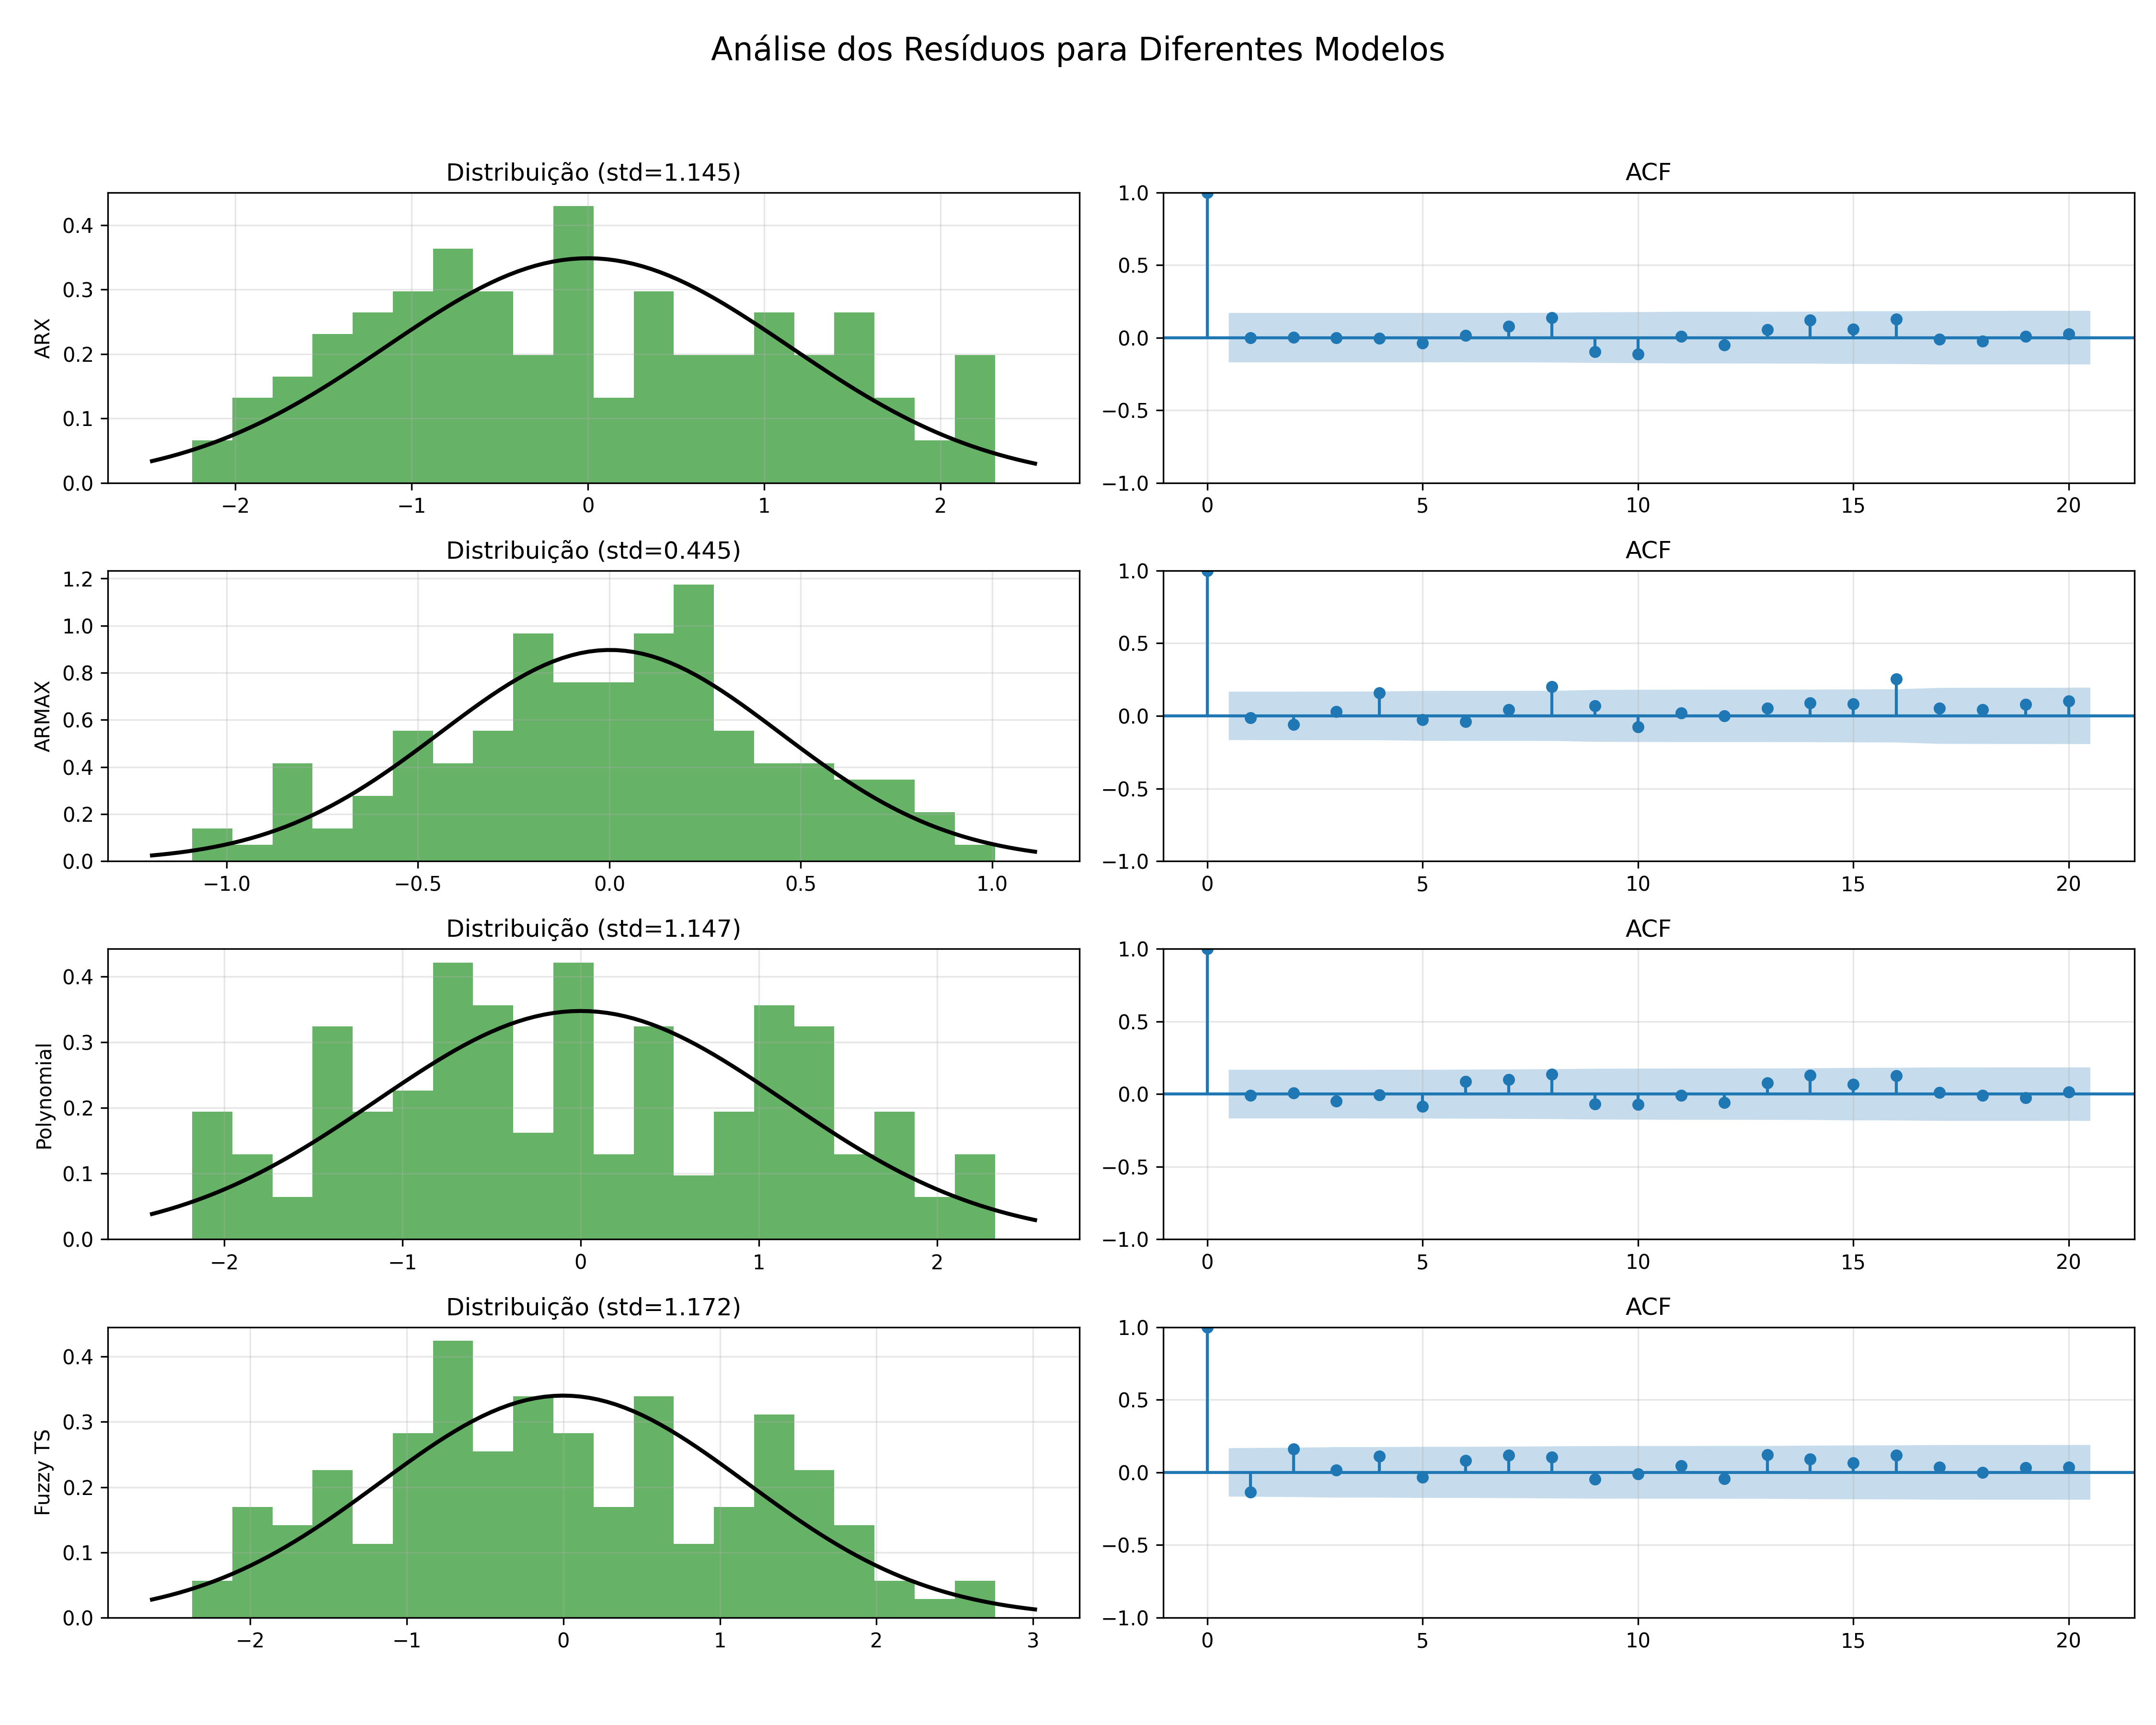
\includegraphics[width=\textwidth]{../analise_residuos.png}
    \caption{Análise estatística e de autocorrelação dos resíduos para os modelos estimados.}
    \label{fig:residuos}
\end{figure}

\subsection{Comparação de Desempenho e Conclusão}
A validação final foi realizada comparando o Erro Quadrático Médio (RMSE) em simulação livre (free run), além de predições de 1 passo e 5 passos à frente.

\begin{table}[H]
    \centering
    \caption{Comparativo de Desempenho no Conjunto de Validação}
    \begin{tabular}{lcccc}
        \toprule
        \textbf{Modelo} & \textbf{RMSE (Livre)} & \textbf{RMSE (1-Passo)} & \textbf{RMSE (5-Passos)} & \textbf{Custo Sinc.} \\
        \midrule
        ARX         & 5.2970 & 7.9523 & 5.9576 & 5.4273 \\
        \textbf{ARMAX} & \textbf{0.4774} & \textbf{0.4772} & \textbf{0.4773} & \textbf{0.4774} \\
        Polinomial  & 1.9653 & 1.3692 & 1.6407 & 2.1927 \\
        Fuzzy       & 1.5601 & 1.5060 & 1.5392 & 1.7247 \\
        \bottomrule
    \end{tabular}
    \label{tab:resultados}
\end{table}

\textbf{Conclusão:}
O modelo \textbf{ARMAX} demonstrou ser o mais adequado para o sistema. Ele apresentou, de forma consistente, o menor erro em todos os cenários de predição, destacando-se principalmente na simulação livre (RMSE de 0.4774 contra 1.56 do segundo melhor, o Fuzzy).

A Figura \ref{fig:validacao} ilustra visualmente a superioridade do modelo ARMAX em seguir a dinâmica da temperatura $T_4$ ao longo do tempo, enquanto o modelo ARX divergiu significativamente e os modelos não-lineares apresentaram ruído ou oscilações maiores.

\begin{figure}[H]
    \centering
    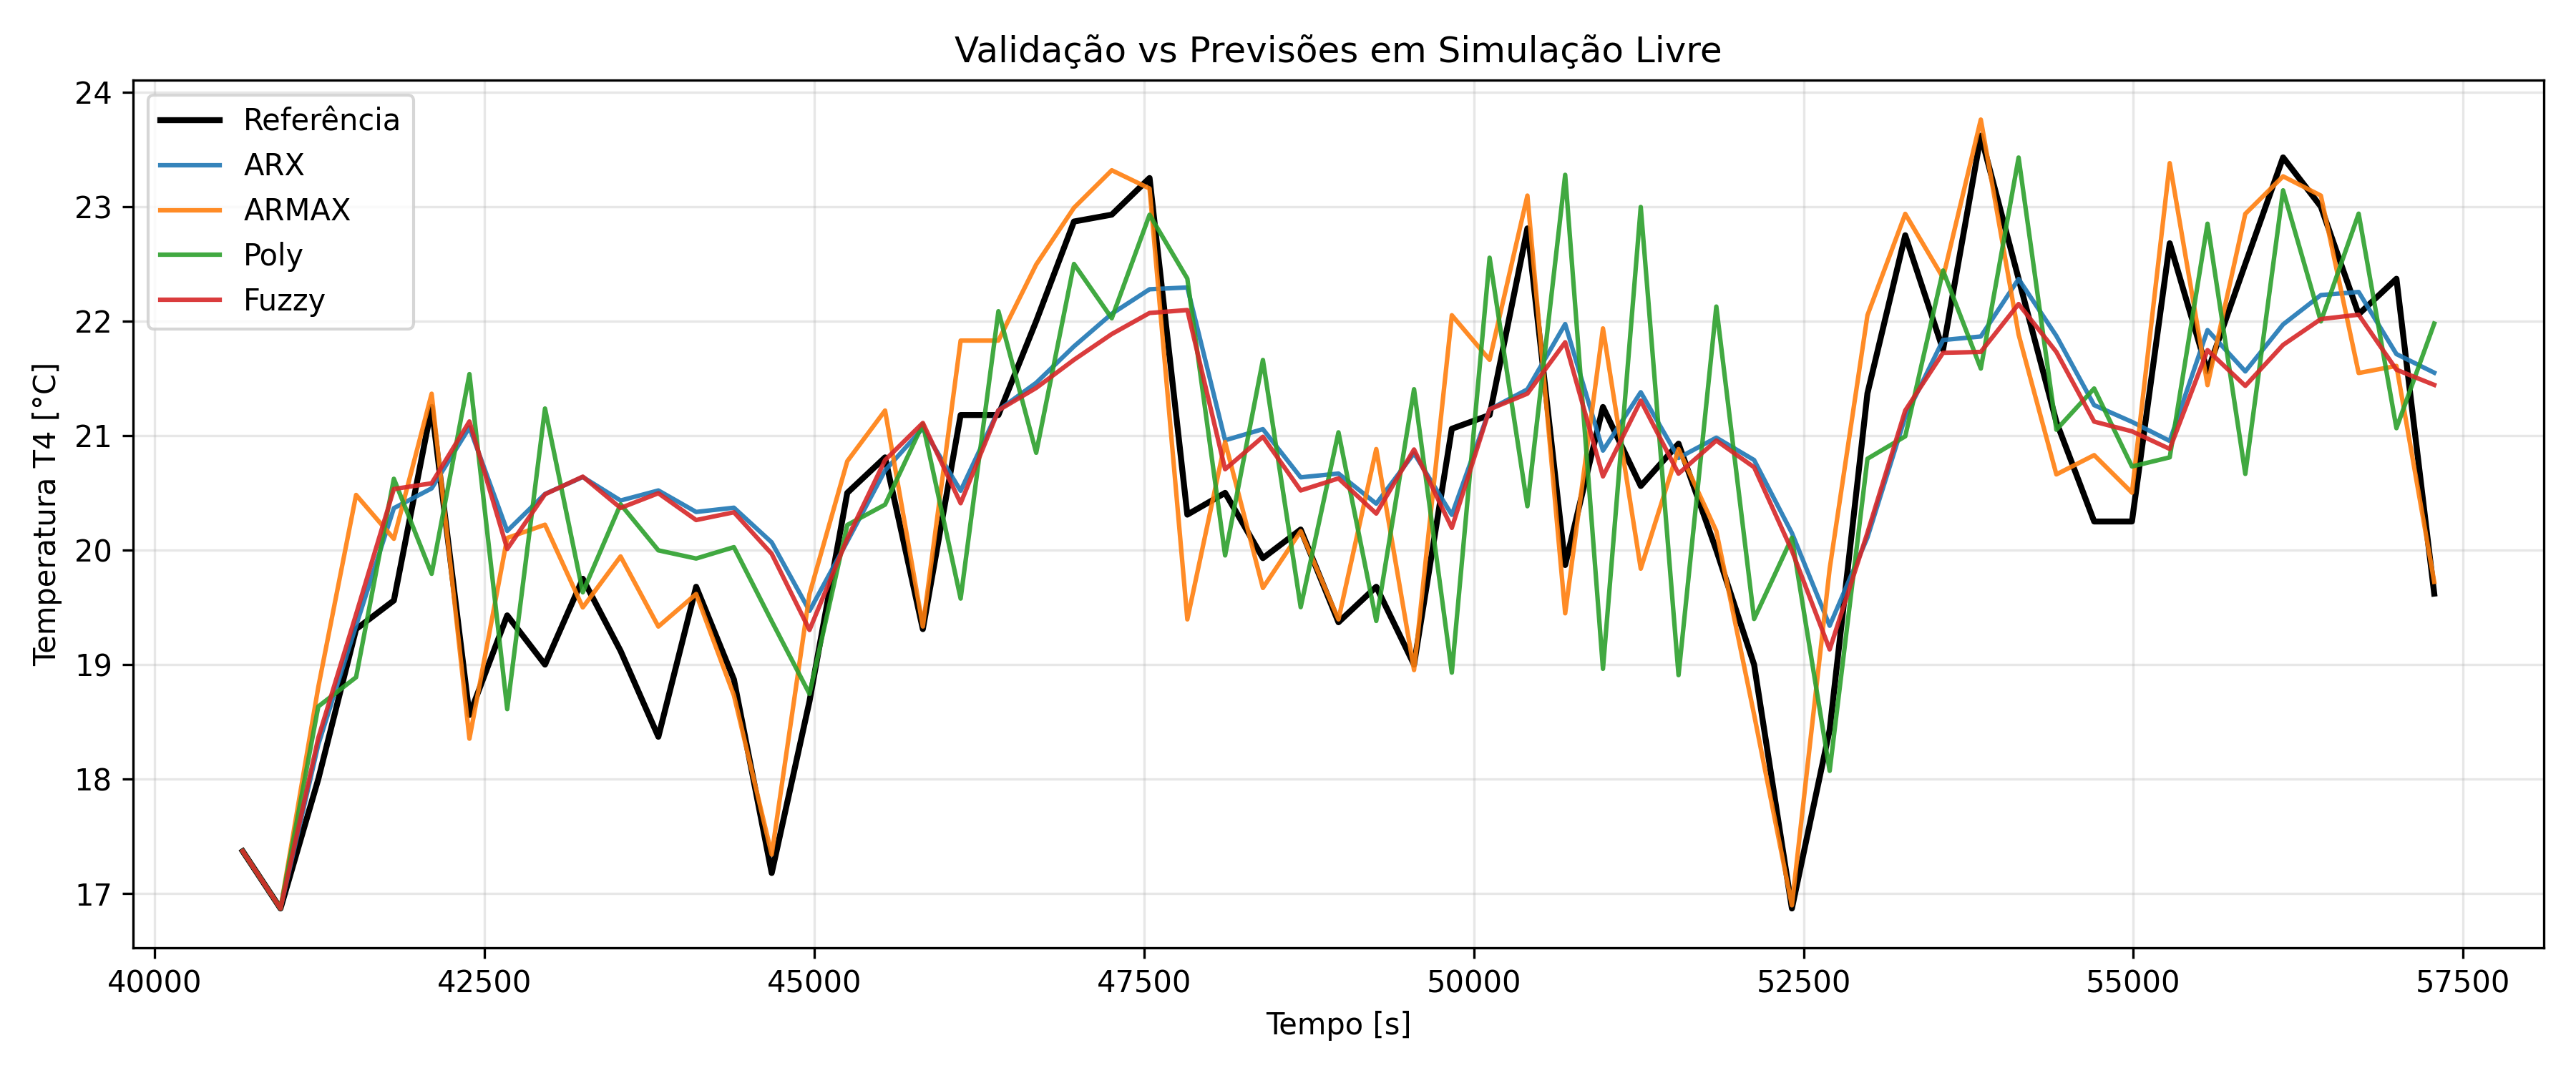
\includegraphics[width=\textwidth]{../validacao.png}
    \caption{Comparação entre a referência (dados reais) e a simulação livre dos modelos.}
    \label{fig:validacao}
\end{figure}

\end{document}